\section{Implémentation}

\begin{figure}[ht]
  \centering
  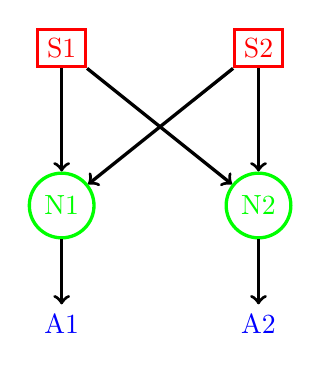
\begin{tikzpicture}[scale=0.5]
 \tikzset{directed/.style={->}} 
  \node[color=blue] (A1) at (0,0) {A1};
  \node[color=blue] (A2) at (5,0) {A2};
  \node[draw, circle, very thick, color=green] (N1) at (0,3) {N1};
  \node[draw, circle, very thick, color=green] (N2) at (5,3) {N2};
  \node[draw, very thick, color=red] (S1) at (0,7) {S1};
  \node[draw, very thick, color=red] (S2) at (5,7) {S2};
  \draw[very thick, directed] (S1) -- (N1);
  \draw[very thick, directed] (S2) -- (N1);
  \draw[very thick, directed] (S1) -- (N2);
  \draw[very thick, directed] (S2) -- (N2);
  \draw[very thick, directed] (N1) -- (A1);
  \draw[very thick, directed] (N2) -- (A2);
\end{tikzpicture}

  \caption{Réseau de neurone à deux neurones}
  \label{graphInit}
\end{figure}

Nous pouvons voir sur le schéma \ref{graphInit} que trois types d'objets sont
présents dans notre conception d'un réseau de neurones:\\
\begin{description}
  \item[Les stimuli] Réalisés en rouge sur le schéma, ils génèrent les signaux
    qui activent les premiers neurones et ainsi active le réseau
  \item[Les actions] Affichés en bleu sur le schéma, elles sont les sorties de
    notre système, elles correspondent à la décision effectué par notre réseau
  \item[Les neurones] Cœur même du réseau, ils sont là pour effectuer la prise
    de décision en fonction des entrées qu'ils possèdent.
\end{description}


Ces trois éléments sont donc la base de notre réseau, cependant nous avons
décidé de rendre générique notre réseau et ainsi notre réseau stockera une liste
de stimulus et de réaction.

Il a ensuite fallu déterminer la façon de parcourir tous les neurones pour les
mettre à jour. Cette réflexion a fait émerger diverses techniques cependant deux
avaient un effet similaire avec une base commune (les stimuli sont le départ du
calcul du réseau) mais modifiaient la façon de considérer chaque
neurone:\\

\begin{enumerate}
  \item La première consistait à considérer que chaque neurone connait les
    neurones qui lui envoient un signal et du coup les interrogent pour
    récupérer les informations nécessaires au calcul de sa sortie
  \item La seconde  considérait que chaque neurone avait en mémoire les différents
      concernés par sa sortie.
\end{enumerate}

Cependant la deuxième solution était bloquante pour l'apprentissage vu que les
poids stockés par le neurone concerne les autres, et du coup nécessitait un lien
autre que ceux accepté par le standard de neurone

[A finir]

Cependant la partie la plus importante du réseau de neurone se situe au niveau
des neurones. Nous nous sommes donc demandé ce qui était intrinsèque au
fonctionnement de l'entité et ce qui relevé de la particularité de notre réseau.

Après réflexion nous sommes arrivé à déterminer comme cœur du neurone, les
parties suivantes:\\

\begin{description}
  \item[Nom] Nous avons décidé d'attribuer à chaque neurone un nom. Ce dernier
    est utilisé au moment de l'attribution
\end{description}
